\documentclass[12pt,twoside]{article}
\usepackage[dvipsnames]{xcolor}
\usepackage{tikz,graphicx,amsmath,amsfonts,amscd,amssymb,bm,cite,epsfig,epsf,url}
\usepackage[hang,flushmargin]{footmisc}
\usepackage[colorlinks=true,urlcolor=blue,citecolor=blue]{hyperref}
\usepackage{amsthm,multirow,wasysym,appendix}
\usepackage{array,subcaption} 
% \usepackage[small,bf]{caption}
\usepackage{bbm}
\usepackage{pgfplots}
\usetikzlibrary{spy}
\usepgfplotslibrary{external}
\usepgfplotslibrary{fillbetween}
\usetikzlibrary{arrows,automata}
\usepackage{thmtools}
\usepackage{blkarray} 
\usepackage{textcomp}
\usepackage[left=0.8in,right=1.0in,top=1.0in,bottom=1.0in]{geometry}
\usepackage{graphics}
\usepackage{pdfpages}
\begin{document}


\section{Introduction}
\begin{center}
{\large{\textbf{Homework 5}} } \vspace{0.2cm}\\
Due October 31 at 11 pm
\\
\end{center}

\begin{enumerate}

\item (Spider on a wall) There's a spider living on a wall of your living room that has a painting behind which the spider likes to hide. Figure~\ref{fig:wall} shows a diagram of the wall; it is 10 feet high and 10 feet wide.

After observing the spider for a while you determine that (1) it spends twice the time behind the painting than on the rest of the wall, (2) it never crawls on the painting or leaves the wall, (3) if it is not behind the painting then it is equally likely to be anywhere on the wall. Since you cannot see it behind the painting, you assume that when it is there it is also equally likely to be at any spot.

\begin{enumerate}
\item Model the position of the spider as a bivariate random variable and give its pdf.
\subitem
Lets use what we know to our advantage. The probability that the spider is behind the painting is $P(Behind \ Painting)=\frac{2}{3}$ and $P(Behind \ Painting)^C=\frac{1}{3}$. We know that the area of the wall that is behind the painting is defined by a $2x2$ square, so the area is $4$. To calculate our pdf, we can use this fact to our advantage, as if we integrate from 4-6 on the horizontal axis, $x$, and 6-8 on the vertical axis, $y$, we will need the probability to equal $\frac{2}{3}$. Lets show this property:

$$
    \int_6^8 \int_4^6 cdxdy = \frac{2}{3} \rightarrow 4c = \frac{2}{3} \rightarrow c= \frac{1}{6}
$$
We have found that the probability of being in any given range of the painting is equal to the integral of $\frac{1}{6}$ along that interval, which is the same as dividing the probability of being in an area, by the area, $\frac{2/3}{4}$. We, we can perform the shortcut to calculate the probability of the spider being on any interval of the wall that is not the painting. We know that we have probability of $\frac{1}{3}$ of being on the wall and not behind the painting, and there are 24 squares on the wall that are not on the painting, that each have area of 4. Therefore, we do the following computation:
$$
    \frac{\frac{1}{3}}{24\times 4} = \frac{1}{288}
$$
This is the same as taking the integral of all possible ranges and setting it equal to the 1/3. Therefore, we have our pdf:
$$
    \begin{cases}
    \text{for any } 4 < x < 6 \text{ and } 6 < y < 8 & \frac{1}{6}\\
    \text{for any } 0 < x < 10 \text{ and } 0 < y < 6 & \frac{1}{288}\\
    \text{for any } 0 < x < 10 \text{ and } 8 < y < 10 & \frac{1}{288}\\
    \text{for any } 0 < x < 6 \text{ and } 6 < y < 8 & \frac{1}{288}\\
    \text{for any } 8 < x < 10 \text{ and } 6 < y < 8 & \frac{1}{288}\\
    \text{otherwise } & \frac{1}{288}
    \end{cases}
$$

\item Compute the pdf of the height at which the spider is located and sketch it.
\subitem
We can compute the pdf of the height ($y$) for which the spider is at by computing the marginal pdf of $y$, where we integrate over $x$.
\begin{equation}
    \begin{split}
    \begin{cases}
        \text{ for any } 0 < y < 6 & \int_0^{10} \frac{1}{288}dx = \frac{10}{288} \\
        \text{ for any } 6 < y < 8 & \frac{4}{5} \times \int_0^{10} \frac{1}{288}dx +\frac{1}{5} \times \int_0^{10} \frac{1}{6}dx = \frac{312}{864} \\
        \text{ for any } 8 < y < 10  & \int_0^{10} \frac{1}{288}dx = \frac{10}{288} \\
        \text{otherwise } & 0
        \end{cases}
    \end{split}
\end{equation}
The pdf would then look like the following:

\begin{figure}[h!]
    \centering
    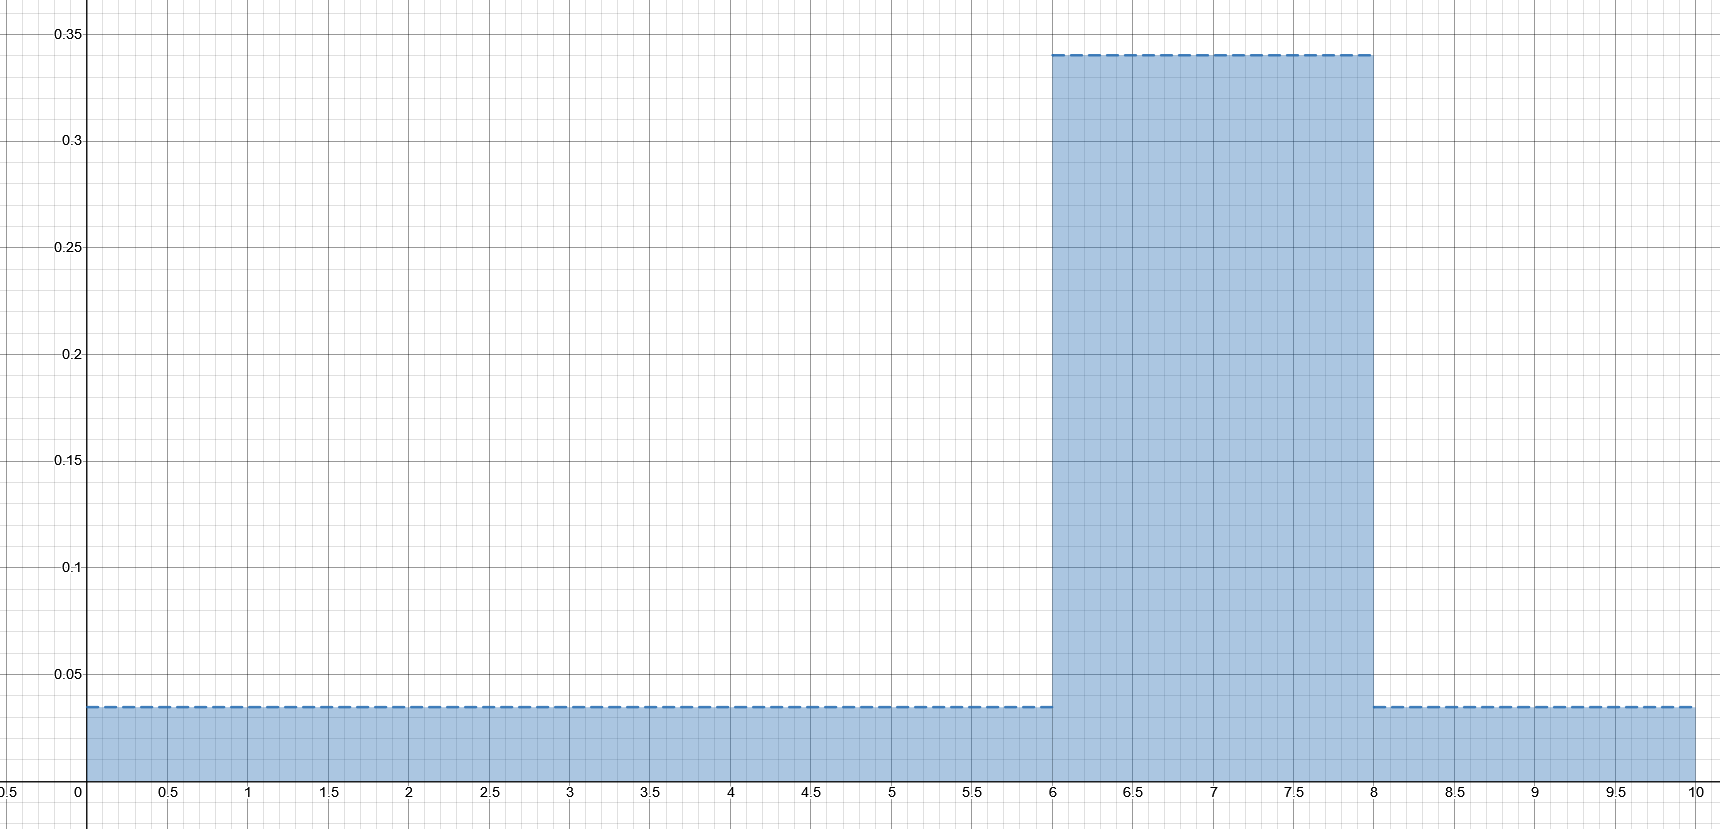
\includegraphics[scale=.3]{desmos 1002 hw5 1.b.png}
    \caption{PDF of Height (y)}
    \label{fig:my_label}
\end{figure}
We can integrate to make sure that this is a valid pmf:
$$
\int_o^6\int_0^{10} \frac{1}{288}dxdy + \frac{4}{5} \times \int_6^8 \int_0^{10} \frac{1}{288}dxdy + \frac{1}{5} \times \int_6^8 \int_0^{10} \frac{1}{6}dxdy + \int_8^{10} \int_0^{10} \frac{1}{288}dxdy  = 1 
$$
Therefor we have a valid pmf.
\item Compute the conditional cdf of the height at which the spider is located, given that you can see it (i.e. it's not under the painting) and sketch it. 
\subitem
If we can see the spider, it cannot be on the painting, and we know that it canot be on the interval of $4 < x < 6 \text{ and } 6 < y < 8$. We can compute the conditional probability, by with the following operation: $$ Conditional \ Probability= \frac{Joint \ Probability}{Marginal \ Probability}$$. We know that in this case, the marginal probability is just $\frac{1}{3}$, the probability that the spider is not behind the painting (by virtue of problem statement). Therefore, we must calculate the joint probability:
\begin{equation}
    \begin{split}
        Joint = \int_0^6 \frac{10}{288}dy + \frac{4}{5} \times \int_6^8 \frac{10}{288}dy + \int_8^{10} \frac{10}{288}dy
    \end{split}
\end{equation}
\end{enumerate}
Here we've already integrated over x, and are integrating over y. We can clearly see that its less likely that the spider is at height $6 < y < 8$ as we know that the spider is not behind the painting, and that leaves only 4 other $2x2$ squares in that row where the spidre could be.
$$
    \begin{cases}
     where \ 0 < y < 6 & \frac{30}{288} \times y\\
     where \ 6 < y < 8 & \frac{30}{288} \times 6 + \frac{24}{288} \times (y-6)\\
     where \ 8 < y < 10 & \frac{30}{288} \times 6 + \frac{24}{288} \times 2 + \frac{30}{288} \times (y-8)\\
    \end{cases}
$$
\begin{figure}[h!]
    \centering
    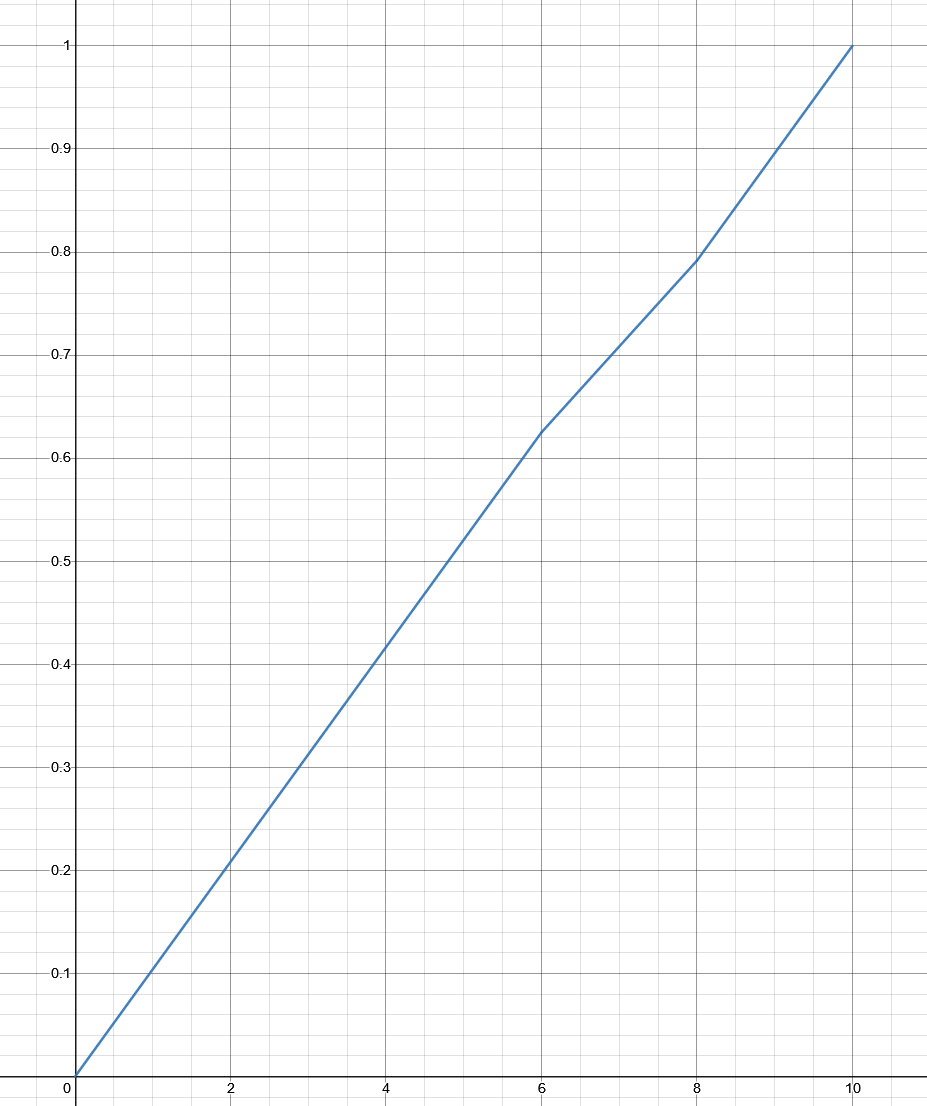
\includegraphics[scale=.4]{desmos 1002 hw5 1.c.png}
    \caption{Conditional CDF}
    \label{fig:my_label}
\end{figure}

\newpage 

\item (Frog)
A frog lives in a garden where there are two ponds. It spends 1/4 of its time in the large pond and the rest in the small pond. When it is in either of the ponds, we model its position as uniformly distributed. 
\begin{enumerate}
\item What is the joint pdf of the vector that indicates the position of the frog in the diagram?
\subitem
Lets call our horizontal axis, $x$, and our vertical axis, $y$. We know that the frog spends $\frac{1}{4}$ of its time in the big pond, which is a $10\times10$ rectangle with $area=100$. Therefore, the probability of the frog being on any interval is equal to:
$$
    \int_0^{10} \int_0^{10} cdydx = \frac{1}{4} \rightarrow 100c = \frac{1}{4} \rightarrow c = \frac{1}{400} \rightarrow \text{ same as }\frac{\frac{1}{4}}{100} = \frac{1}{400}
$$
Likewise, for the frog being in the smaller pond the probability is $\frac{3}{4}$ and therefore:
$$
    \int_{12}^{17} \int_0^5 cdydx = \frac{3}{4} \rightarrow 25c = \frac{3}{4} \rightarrow c = \frac{3}{100} \rightarrow \text{ same as }\frac{\frac{3}{4}}{25} = \frac{3}{100}
$$
We now have our pdf:
$$
    \begin{cases}
    \text{for any } 0 < x < 5 \text{ and } 12 < y < 17 & \frac{3}{100}\\
    \text{for any } 0 < x < 10 \text{ and } 0 < y < 10 & \frac{1}{400}\\
    otherwise & 0\\
    \end{cases}
$$

\item What is the marginal pdf of the horizontal position of the frog (i.e. its position on the horizontal axis)? Sketch the pdf. 
\subitem
To compute the marginal pdf of the hortizontal position of the frog, we integrate over what we don't care about, in this case, the vertical axis, $y$. We need to split our hortizontal axis, $x$, into two groups, $x<5$ and $x>5$.
$$
    \int_5^{10} \int_0^{10}\frac{1}{400}dydx = \int_{5}^{10}\frac{10}{400}dx = \frac{1}{8} \text{ when } x>5$$ 
$$
    \int_{0}^5 \int_0^{10}\frac{1}{400}dydx + \int_0^5 \int_{12}^{17} \frac{3}{100}dydx = \frac{7}{8} \text{ when } x < 5 \\ 
$$
We need to divide by the area, to get our pdf. 
%For $x<5$ we have two rectangles, whos areas sum to $(5*5) + (5*10) = 75 $, and for $x>5$ we have one $5*10$ rectangle whos area is 50.% 
We adjust the probabilities to calculate the pdf like so $P(0<x<5) = \frac{\frac{7}{8}}{5}=\frac{7}{40}$ and $P(5<x<10)=\frac{\frac{1}{8}}{5}=\frac{1}{40}$\\

Therefore the marginal PDF of the horizontal position of the frog is:
$$
    \begin{cases}
    when \ 0<x<5 & 7/40\\
    when \ 5<x<10 & 1/40
    \end{cases}
$$
\begin{figure}[h!]
    \centering
    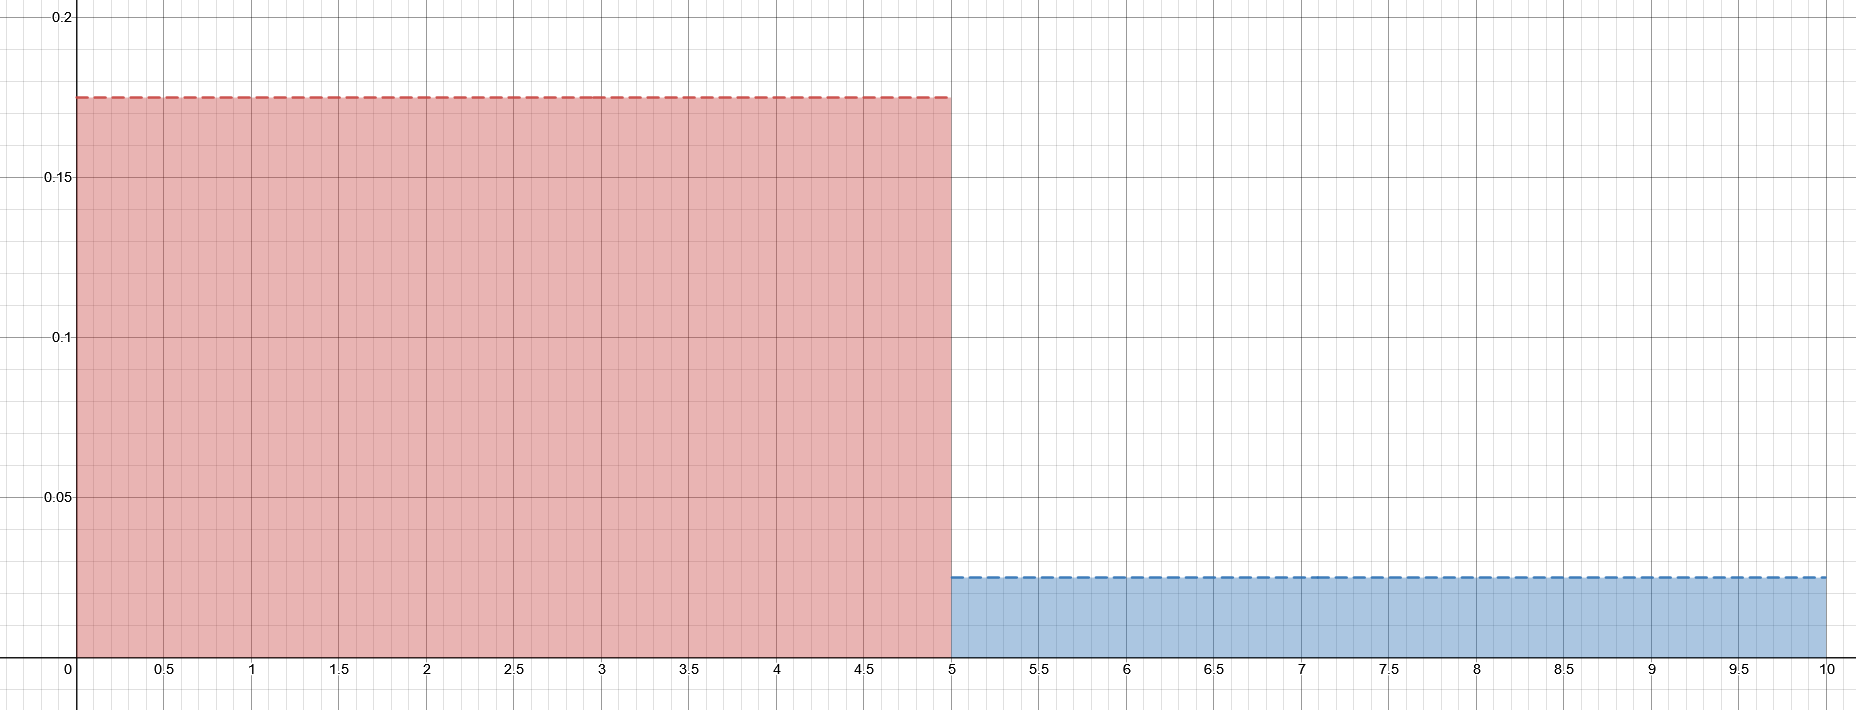
\includegraphics[scale=.3]{desmos 1002 hw5 2.b.png}
    \caption{2.b) Marginal PDF of Position (x)}
    \label{fig:my_label}
\end{figure}

\newpage

\item If we know that the horizontal position of the frog is 3, what is the conditional pdf of its vertical position given this information? Sketch the pdf. 
\subitem
We know that 
$$
    Conditional \ = \frac{Joint}{Marginal}
$$
Since we already have found the joint, lets calculate the marginal.

\begin{equation}
    \begin{split}
        \text{Marginal of x, integrate over y: }\int_0^{10} \frac{1}{400}dy + \int_{12}^{17}\frac{3}{100}dy = \frac{7}{40}
    \end{split}
\end{equation}

We can divide the two with our formula to obtain:
$$
    \begin{cases}
    \text{for any }  12 < y < 17 & \frac{12}{70} \\
    \text{for any }  0 < y < 10 & \frac{1}{70}\\
    otherwise & 0\\
    \end{cases}
$$
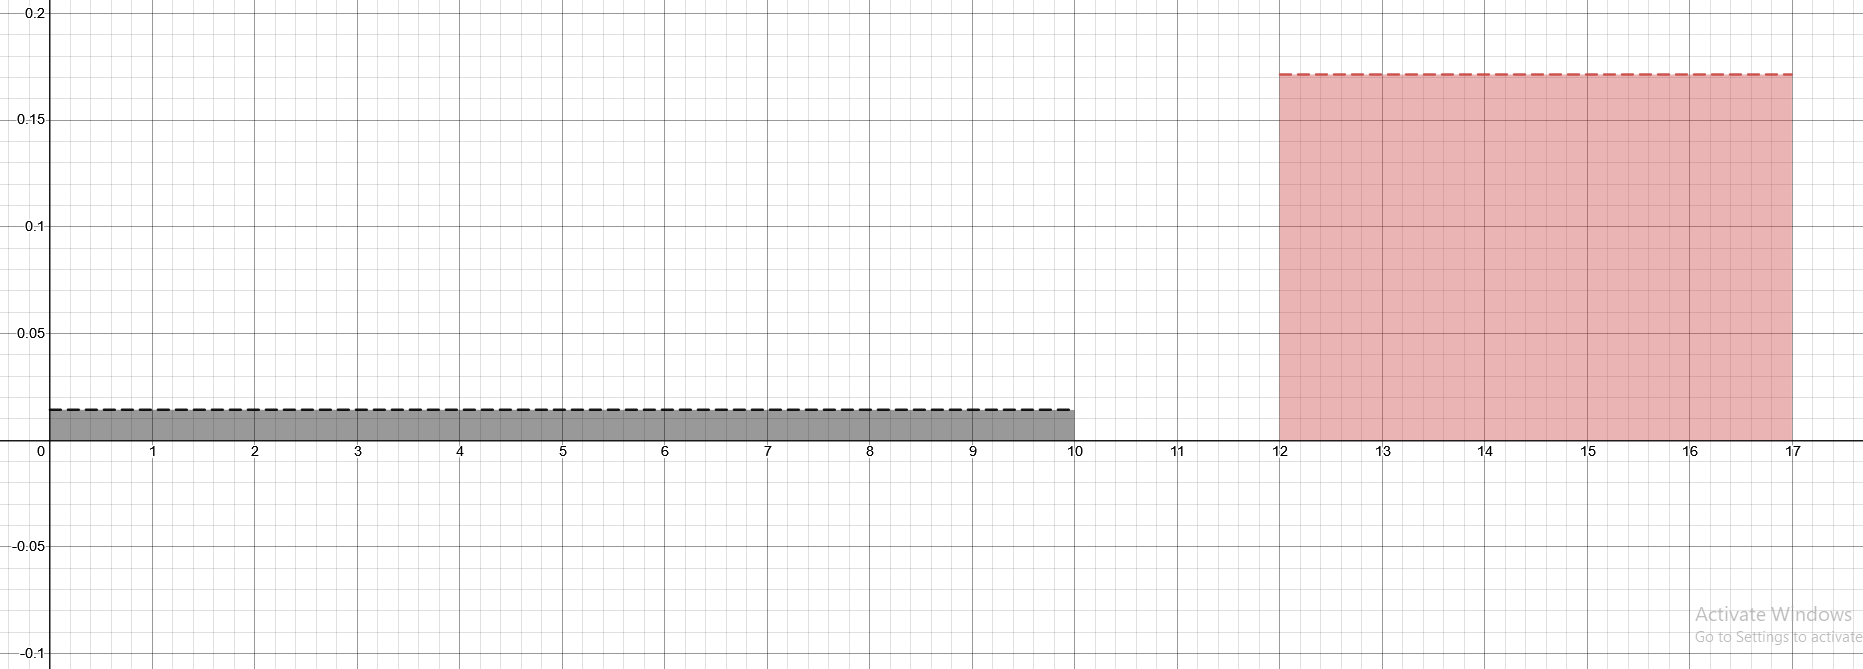
\includegraphics[scale=.25]{desmos 1002 hw5 2.c.png}

\item Is the vertical position of the frog independent from the horizontal position of the frog? Justify your answer mathematically. 
\subitem
We know if the vertical position of the frog is independent of the horizontal position, we will have the following equality:

$$
    f_y(y) = f_{y,x}(y|x=3)
$$
What we find is that we do not have the equality, and that the two positions are not independent. We do so by computing the marginal of $y$
$$
    \begin{cases}
    \text{for any } 0 < y < 10 & \frac{1}{400}\\
    \text{for any } 12 < y < 17 & \frac{12}{400}\\
    \text{otherwise } & 0
    \end{cases}
$$
Which does not equal the conditional probability that we computed above. $P(y|x=3)$ as follows:
$$
    \begin{cases}
    \text{for any }  12 < y < 17 & \frac{12}{70} \\
    \text{for any }  0 < y < 10 & \frac{1}{70}\\
    otherwise & 0\\
    \end{cases}
$$
\item Is the vertical position of the frog conditionally independent from the horizontal position given the event \emph{the frog is in the small pond}? Justify your answer mathematically. 

\subitem

Yes! The vertical position of the frog is conditionally independent from the horizontal position, given that we know that the frog is in the small pond. This is because if the frog is in the small pond, it has a uniform distribution across its x and y ranges, and therefore any information about the horizontal position, x, does not influence the probability of being in any vertical range y.

$$
    f(x,y|small) = f(x|small)f(y|small)
$$
$$
    \int_0^5 \int_0^5 f(x,y|small)dxdx = \int_0^5f(x|small)dx \int_{12}^{17}f(y|small)dy
$$
$$
    \frac{1}{25} = \frac{1}{5}\times \frac{1}{5}
$$
And this equality holds!

\end{enumerate}
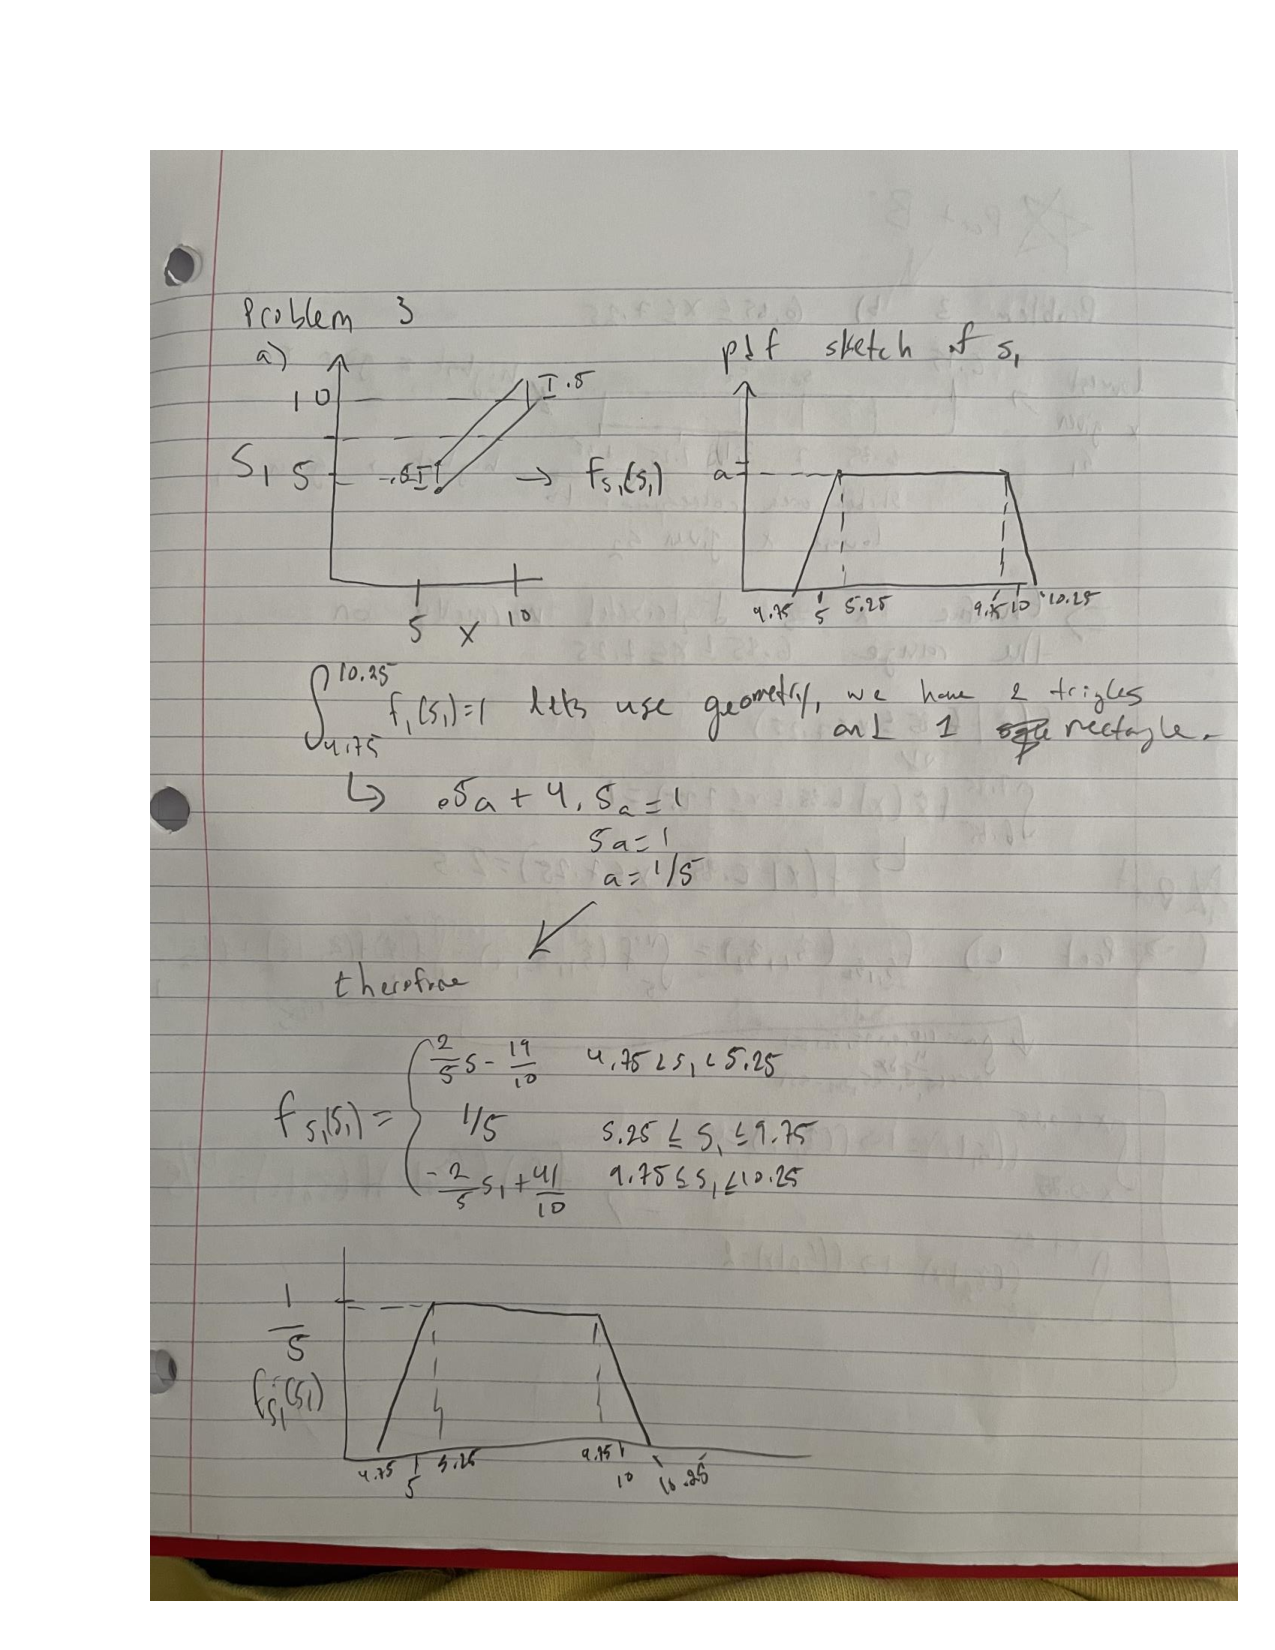
\includepdf[pages=-]{HW5 pics.pdf}
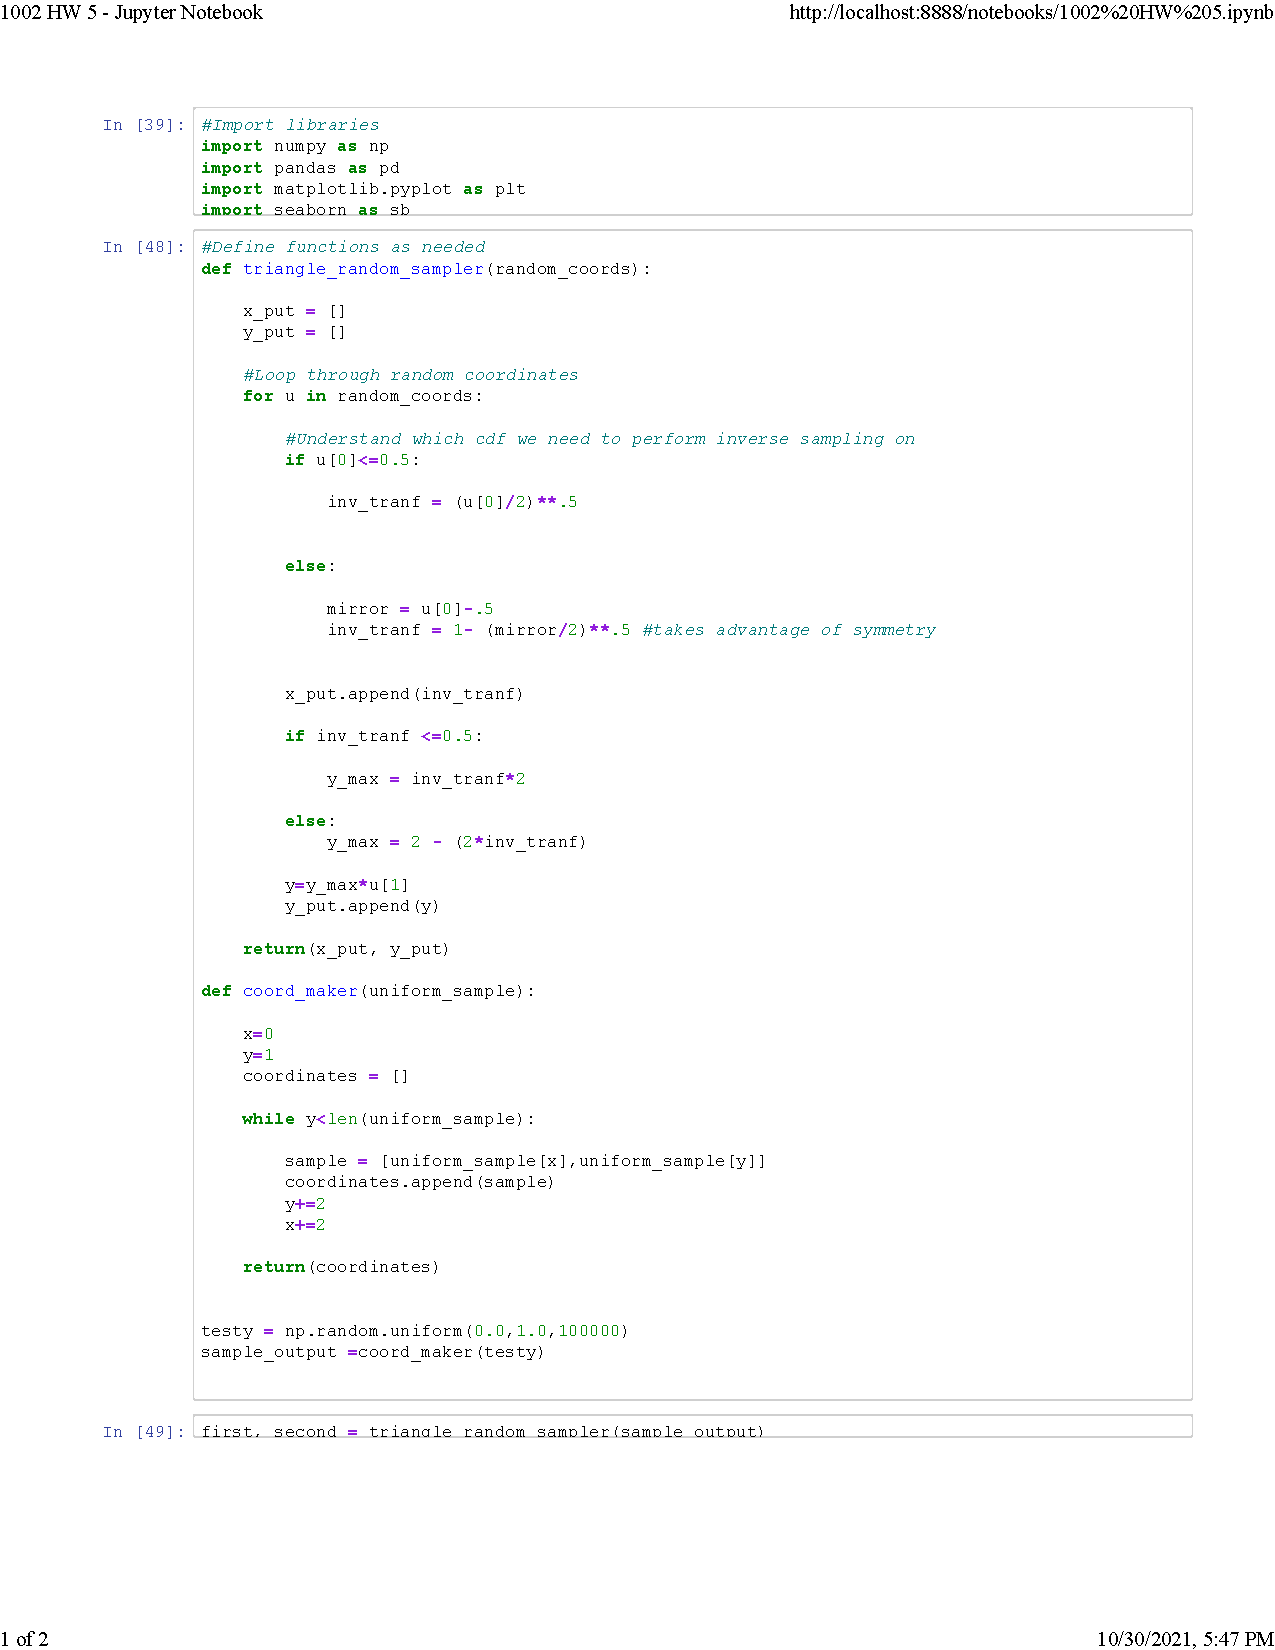
\includepdf[pages=-]{code.pdf}
\end{enumerate}
\end{document}
